\chapter{Analítica con Athena}
Analytics es una API FastAPI que consulta Amazon Athena. El servicio inicia la consulta, espera el resultado y devuelve las filas en formato JSON. La ubicación de los resultados se configura con \texttt{ATHENA\_OUTPUT\_BUCKET}.

Los datos de ASTRA CLOUD se guardan en distintos servicios: el catálogo en PostgreSQL, la información social en MySQL y las interacciones en MongoDB. Los contenedores de carga los convierten en archivos CSV y los suben a Amazon S3. Después, AWS Glue registra su estructura y Athena los consulta sin afectar las bases de datos que usa la aplicación.

\section{Panel de analítica en la aplicación desplegada}
El panel de analítica está disponible en la ruta \path{/analytics} para los usuarios que iniciaron sesión. Desde esta sección se consultan los indicadores generales de la plataforma: cantidad de películas, usuarios, clubes, salas e interacciones. También se muestran los géneros más vistos, los actores populares y los clubes con mayor actividad, como se observa en la Figura~\ref{fig:analytics-dashboard}. Durante las pruebas notamos que el campo \emph{Rating Promedio} aparecía como \texttt{NaN}, por lo que no lo tomamos como un valor válido. Este problema queda pendiente de revisión, ya que puede estar relacionado con el dato que recibe el frontend o con la forma en que se procesa antes de mostrarlo.

\begin{figure}[H]
  \centering
  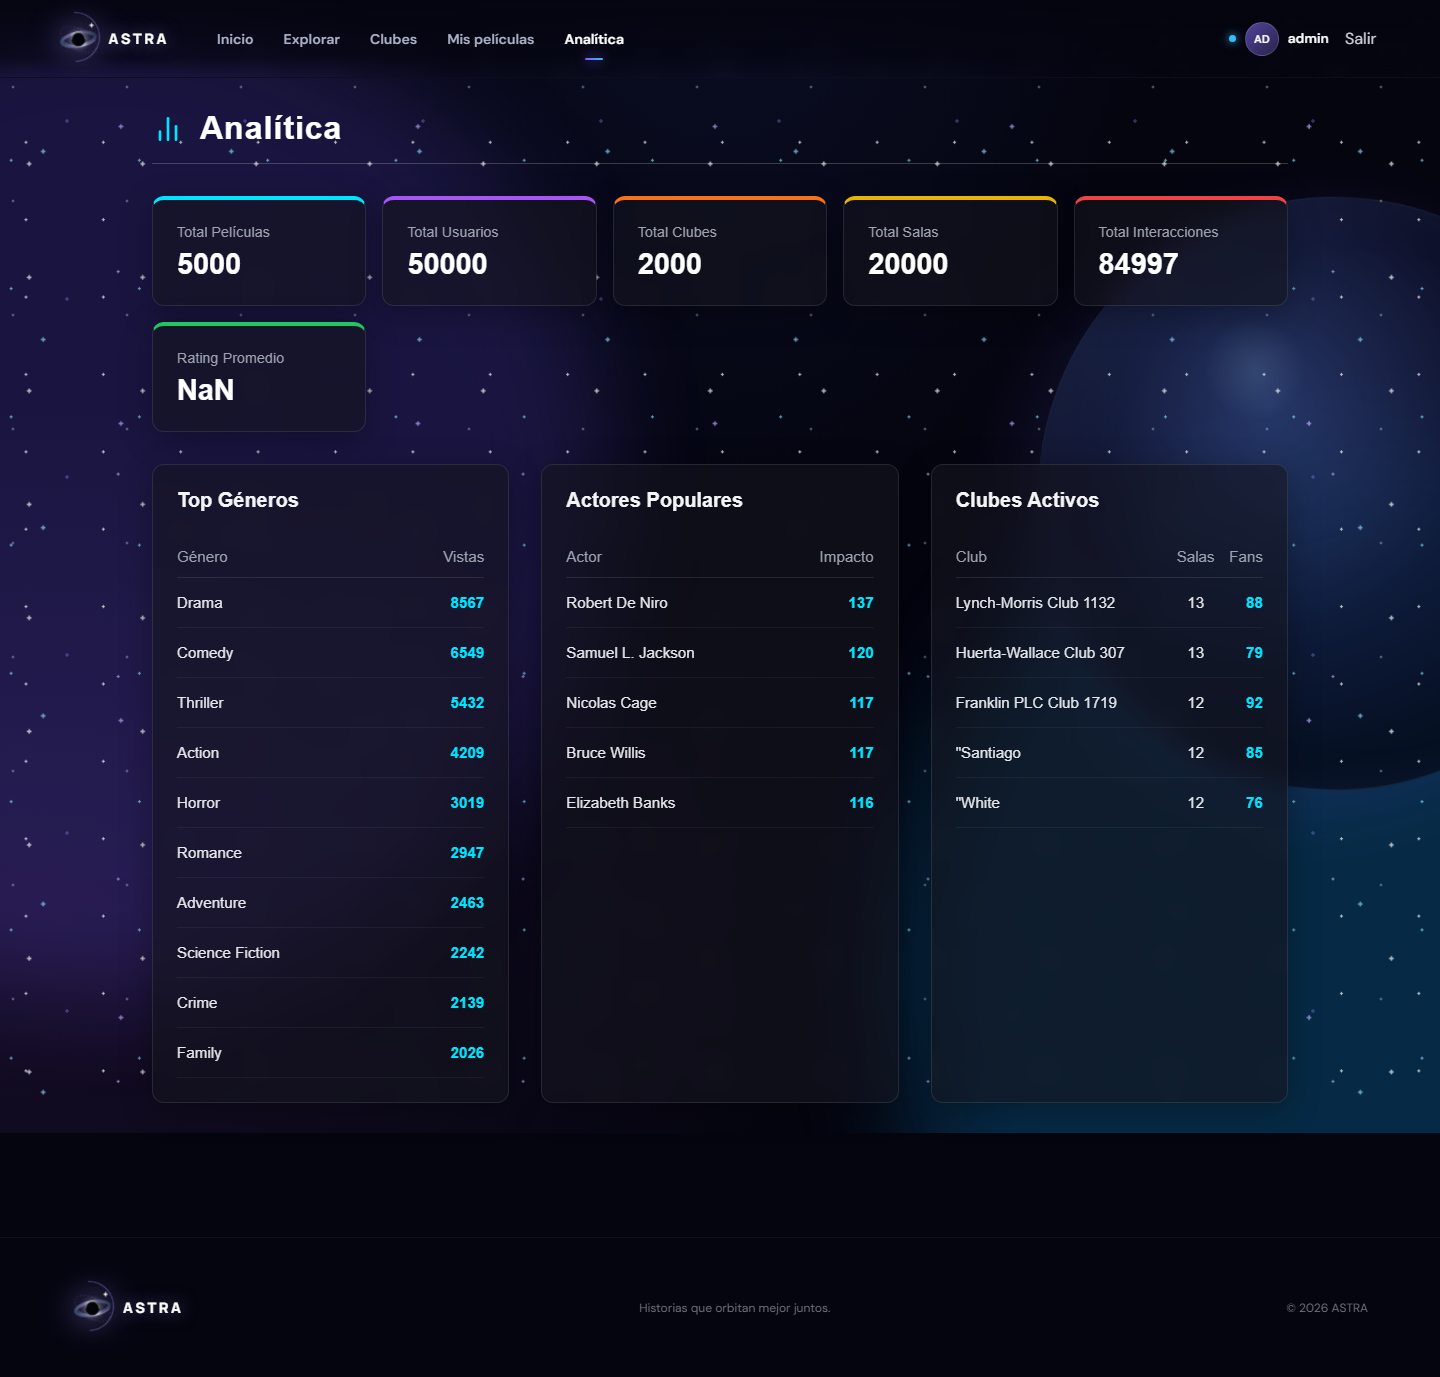
\includegraphics[width=.96\textwidth]{evidence/analytics/analytics-dashboard-kpis-tables.png}
  \caption{Panel de analítica desplegado con KPIs y tablas de géneros, actores y clubes.}
  \label{fig:analytics-dashboard}
\end{figure}

\section{Consultas analíticas en AWS Athena}
\lstset{language=SQL,basicstyle=\ttfamily\scriptsize,breaklines=true,frame=single,framesep=5pt,backgroundcolor=\color{black!3},keywordstyle=\color{utecblue}\bfseries,commentstyle=\color{gray}\itshape,captionpos=b}

\subsection*{Consulta 1: Engagement por género}
Para saber qué géneros  tienen más participación, reunimos los datos de \texttt{genre}, \texttt{movie\_genre}, \texttt{movie}, \texttt{watch\_rooms} e \texttt{iteraction}. La consulta obtiene el total de películas, salas, rating promedio, reseñas y likes de cada categoría.

\begin{lstlisting}[caption={Consulta SQL de engagement por género en Athena},label={lst:athena-engagement-genero}]
WITH movie_stats AS (
    SELECT m.id as movie_id, m.rating as avg_rating,
        (SELECT COUNT(DISTINCT id)
         FROM "astra\_analytics"."watch_rooms"
         WHERE movie_id = CAST(m.public_id AS VARCHAR)) as watch_rooms,
        (SELECT COUNT(1) FROM "astra\_analytics"."iteraction"
         WHERE movie_id = CAST(m.public_id AS VARCHAR)
           AND partition_0 = 'reviews') as total_reviews,
        (SELECT COUNT(1) FROM "astra\_analytics"."iteraction"
         WHERE movie_id = CAST(m.public_id AS VARCHAR)
           AND partition_0 = 'likes') as total_likes
    FROM "astra\_analytics"."movie" m
)
SELECT g.name as genre_name, COUNT(DISTINCT mg.movie_id) as total_movies,
    SUM(ms.watch_rooms) as total_watch_rooms,
    AVG(ms.avg_rating) as avg_rating, SUM(ms.total_reviews) as total_reviews,
    SUM(ms.total_likes) as total_likes
FROM "astra\_analytics"."genre" g
JOIN "astra\_analytics"."movie_genre" mg ON g.id = mg.genre_id
JOIN movie_stats ms ON mg.movie_id = ms.movie_id
GROUP BY g.name
ORDER BY total_watch_rooms DESC;
\end{lstlisting}

Primero se calculan las métricas de cada película y luego se agrupan por género. Al ejecutar la consulta obtuvimos el resultado de la Figura~\ref{fig:athena-engagement-genero}: Drama concentra 8\,567 \textit{watch rooms}, 8\,495 reseñas y 10\,651 likes; Comedy aparece después con 6\,549 salas.

\begin{figure}[H]
  \centering
  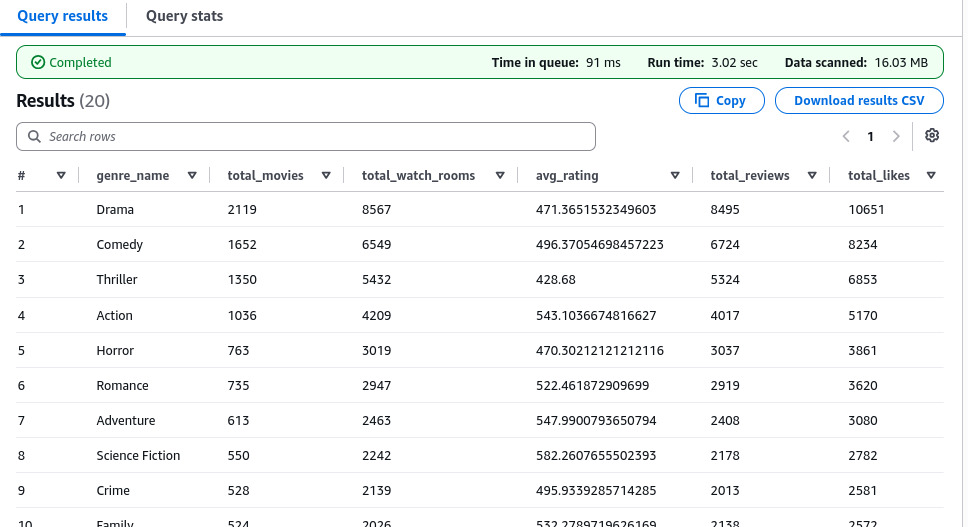
\includegraphics[width=.96\textwidth]{evidence/athena-consulta1-engagement-genero.jpeg}
  \caption{Resultado de la consulta de engagement por género en AWS Athena}
  \label{fig:athena-engagement-genero}
\end{figure}

\clearpage
\subsection*{Consulta 2: Participación de usuarios en la plataforma}
Para conocer qué tanto participan los usuarios, comparamos el total de registrados con quienes se han unido a clubes, participado en \textit{watch rooms} o realizado reseñas. Se usan las tablas \texttt{users}, \texttt{memberships}, \texttt{watch\_participants} e \texttt{iteraction}. \texttt{COUNT(DISTINCT ...)} evita contar más de una vez a un usuario que participa en varias acciones.

\begin{lstlisting}[caption={Consulta SQL de participación de usuarios en Athena},label={lst:athena-participacion-usuarios}]
SELECT
    (SELECT COUNT(1) FROM "astra\_analytics"."users") AS registered_users,
    (SELECT COUNT(DISTINCT user_id)
     FROM "astra\_analytics"."memberships") AS users_in_clubs,
    (SELECT COUNT(DISTINCT user_id)
     FROM "astra\_analytics"."watch_participants") AS users_in_watch_rooms,
    (SELECT COUNT(DISTINCT user_id)
     FROM "astra\_analytics"."iteraction"
     WHERE partition_0 = 'reviews') AS reviewers;
\end{lstlisting}

Como se observa en la Figura~\ref{fig:athena-participacion-usuarios}, Athena devolvió 50\,000 usuarios registrados, 47\,595 usuarios en clubes, 37\,612 participantes en \textit{watch rooms} y 16\,541 revisores.

\begin{figure}[H]
  \centering
  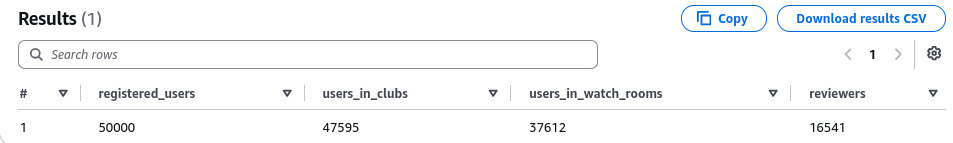
\includegraphics[width=.94\textwidth]{evidence/athena-consulta2-participacion-usuarios.jpeg}
  \caption{Resultado de la consulta de participación de usuarios en AWS Athena}
  \label{fig:athena-participacion-usuarios}
\end{figure}

\subsection*{Consulta 3: métricas de interacción por película}
Para revisar la actividad de cada película, unimos el catálogo, las interacciones y las salas de visualización. La consulta usa \texttt{movie}, \texttt{iteraction} y \texttt{watch\_rooms}, e incluye el identificador público, el título, el rating del catálogo, el promedio de puntuaciones, los likes y la cantidad de salas.

\begin{lstlisting}[caption={Consulta SQL de métricas de interacción por película en Athena},label={lst:athena-metricas-peliculas}]
WITH movie_metrics AS (
    SELECT m.public_id, m.title, m.rating AS catalog_rating,
        (SELECT AVG(CAST(score AS DOUBLE))
         FROM "astra\_analytics"."iteraction"
         WHERE movie_id = CAST(m.public_id AS VARCHAR)
           AND partition_0 = 'reviews') AS avg_user_review_score,
        (SELECT COUNT(1) FROM "astra\_analytics"."iteraction"
         WHERE movie_id = CAST(m.public_id AS VARCHAR)
           AND partition_0 = 'likes') AS likes_count,
        (SELECT COUNT(1) FROM "astra\_analytics"."watch_rooms"
         WHERE movie_id = CAST(m.public_id AS VARCHAR)) AS watch_room_count
    FROM "astra\_analytics"."movie" m
)
SELECT * FROM movie_metrics
ORDER BY watch_room_count DESC
LIMIT 100;
\end{lstlisting}

La consulta ordena las películas por cantidad de salas y muestra las primeras 100 filas. El resultado de la Figura~\ref{fig:athena-metricas-peliculas} incluye títulos como \textit{Contracted: Phase II}, \textit{Getting Even with Dad} y \textit{Rise of the Guardians}, junto con sus identificadores públicos y métricas.

\begin{figure}[H]
  \centering
  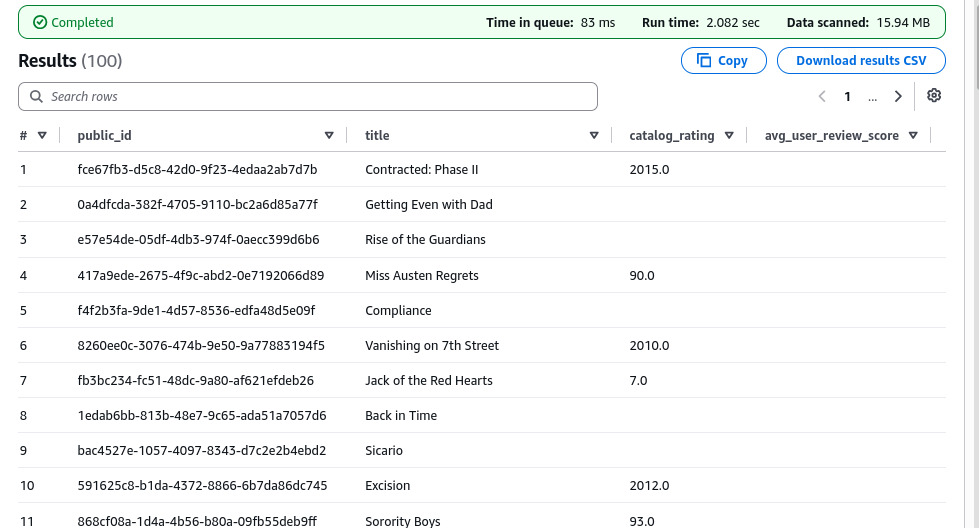
\includegraphics[width=.96\textwidth]{evidence/athena-consulta3-metricas-peliculas.jpeg}
  \caption{Resultado de la consulta de métricas de interacción por película en AWS Athena}
  \label{fig:athena-metricas-peliculas}
\end{figure}

\subsection*{Consulta 4: Nivel de actividad de los clubes}
Para revisar la actividad de los clubes, unimos cada club con sus miembros, las salas creadas y las películas visualizadas. La consulta usa \texttt{clubs}, \texttt{memberships} y \texttt{watch\_rooms}; muestra el nombre del club, sus miembros únicos, salas, relación de actividad y películas diferentes.

\begin{lstlisting}[caption={Consulta SQL de nivel de actividad de clubes en Athena},label={lst:athena-actividad-clubes}]
SELECT c.name AS club_name,
    COUNT(DISTINCT m.user_id) AS member_count,
    COUNT(DISTINCT wr.id) AS total_watch_rooms,
    CAST(COUNT(DISTINCT wr.id) AS DOUBLE)
        / NULLIF(COUNT(DISTINCT m.user_id), 0) AS activity_ratio,
    COUNT(DISTINCT wr.movie_id) AS unique_movies_watched
FROM "astra\_analytics"."clubs" c
LEFT JOIN "astra\_analytics"."memberships" m ON c.id = m.club_id
LEFT JOIN "astra\_analytics"."watch_rooms" wr ON c.id = wr.club_id
GROUP BY c.name
ORDER BY activity_ratio DESC NULLS LAST;
\end{lstlisting}

Los \texttt{LEFT JOIN} incluyen también a los clubes que todavía no  tienen membresías o salas. \texttt{NULLIF} evita una división entre cero cuando un club no registra miembros. La Figura~\ref{fig:athena-actividad-clubes} muestra 1\,712 resultados ordenados por \texttt{activity\_ratio}. Townsend-Wood Club 1456 registra 53 miembros, 11 salas y una relación de actividad de aproximadamente 0.208; Huerta-Wallace Club 307 registra 79 miembros y 13 salas.

\begin{figure}[H]
  \centering
  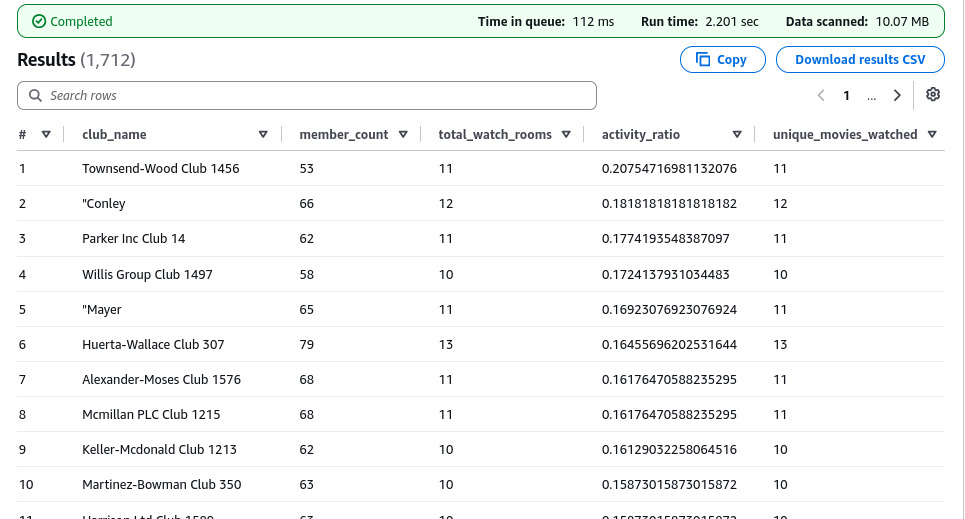
\includegraphics[width=.96\textwidth]{evidence/athena-consulta4-actividad-clubes.jpeg}
  \caption{Resultado de la consulta de actividad de clubes en AWS Athena}
  \label{fig:athena-actividad-clubes}
\end{figure}

\section{Vistas analíticas en AWS Athena}
Además de las consultas, se crearon vistas en Athena para reutilizar datos de distintos componentes de ASTRA CLOUD.

\subsection*{Vista 1: Consolidado analítico de películas}
La vista \texttt{vw\_consolidado\_peliculas} une el catálogo, sus géneros, las salas de visualización y las interacciones. Usa \texttt{movie}, \texttt{movie\_genre}, \texttt{genre}, \texttt{watch\_rooms} e \texttt{iteraction} para mostrar el identificador de película, el título, el género, el total de salas, los likes y el promedio de puntuaciones.

\begin{lstlisting}[caption={Creación de la vista vw\_consolidado\_peliculas},label={lst:athena-vista-consolidado}]
CREATE OR REPLACE VIEW vw_consolidado_peliculas AS
SELECT m.public_id AS movie_id, m.title, g.name AS genre,
    COUNT(DISTINCT w.id) AS total_salas,
    COUNT(i_likes.user_id) AS total_likes,
    AVG(CAST(i_reviews.score AS DOUBLE)) AS promedio_usuarios
FROM "astra\_analytics"."movie" m
LEFT JOIN "astra\_analytics"."movie_genre" mg ON m.id = mg.movie_id
LEFT JOIN "astra\_analytics"."genre" g ON mg.genre_id = g.id
LEFT JOIN "astra\_analytics"."watch_rooms" w
    ON CAST(m.public_id AS VARCHAR) = w.movie_id
LEFT JOIN "astra\_analytics"."iteraction" i_likes
    ON CAST(m.public_id AS VARCHAR) = i_likes.movie_id
    AND i_likes.partition_0 = 'likes'
LEFT JOIN "astra\_analytics"."iteraction" i_reviews
    ON CAST(m.public_id AS VARCHAR) = i_reviews.movie_id
    AND i_reviews.partition_0 = 'reviews'
GROUP BY m.public_id, m.title, g.name;
\end{lstlisting}

La Figura~\ref{fig:athena-vista1-creacion} muestra la Creación de la vista y la Figura~\ref{fig:athena-vista1-consulta}, su consulta. Entre las filas aparecen \textit{Jurassic World}, \textit{Mad Max: Fury Road} y \textit{Terminator Genisys}, con sus géneros, salas y likes. Con esta vista no es necesario repetir las mismas uniones en cada consulta.

\begin{figure}[H]
  \centering
  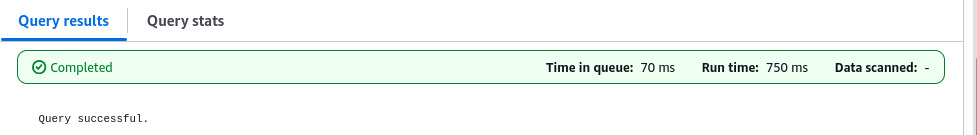
\includegraphics[width=.76\textwidth]{evidence/athena-vista1-creacion.jpeg}
  \caption{Creación de la vista vw\_consolidado\_peliculas en AWS Athena}
  \label{fig:athena-vista1-creacion}
\end{figure}
\begin{figure}[H]
  \centering
  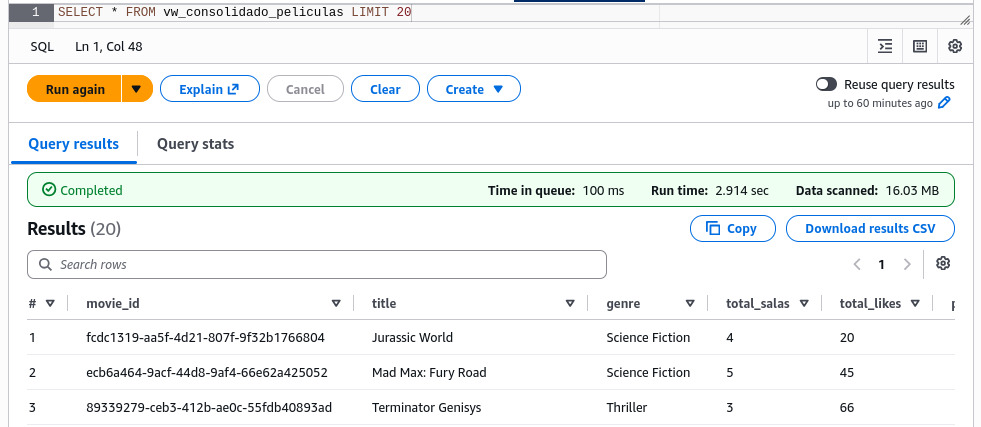
\includegraphics[width=.96\textwidth]{evidence/athena-vista1-consulta.jpeg}
  \caption{Consulta de la vista vw\_consolidado\_peliculas en AWS Athena}
  \label{fig:athena-vista1-consulta}
\end{figure}

\subsection*{Vista 2: Perfil social de usuarios}
La vista \texttt{vw\_perfil\_social\_usuarios} reúne la participación social de cada usuario. Relaciona \texttt{users}, \texttt{memberships} y \texttt{watch\_participants} para mostrar el identificador, username, correo electrónico, clubes unidos y salas en las que participó.

\begin{lstlisting}[caption={Creación de la vista vw\_perfil\_social\_usuarios},label={lst:athena-vista-perfil}]
CREATE OR REPLACE VIEW vw_perfil_social_usuarios AS
SELECT u.id AS user_id, u.username, u.email,
    COUNT(DISTINCT m.club_id) AS clubes_unidos,
    COUNT(DISTINCT wp.watch_room_id) AS salas_participadas
FROM "astra\_analytics"."users" u
LEFT JOIN "astra\_analytics"."memberships" m
    ON CAST(u.id AS VARCHAR) = CAST(m.user_id AS VARCHAR)
LEFT JOIN "astra\_analytics"."watch_participants" wp
    ON CAST(u.id AS VARCHAR) = CAST(wp.user_id AS VARCHAR)
GROUP BY u.id, u.username, u.email;
\end{lstlisting}

La Figura~\ref{fig:athena-vista2-creacion} muestra la Creación de la vista y la Figura~\ref{fig:athena-vista2-consulta}, su consulta. Entre las filas aparece \texttt{jeanmoreno\_3781}, con 4 clubes y 4 salas. Así se puede consultar rápidamente en cuántos clubes y salas participó cada usuario.

\begin{figure}[H]
  \centering
  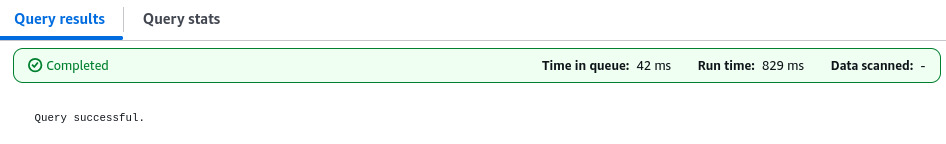
\includegraphics[width=.76\textwidth]{evidence/athena-vista2-creacion.jpeg}
  \caption{Creación de la vista vw\_perfil\_social\_usuarios en AWS Athena}
  \label{fig:athena-vista2-creacion}
\end{figure}
\begin{figure}[H]
  \centering
  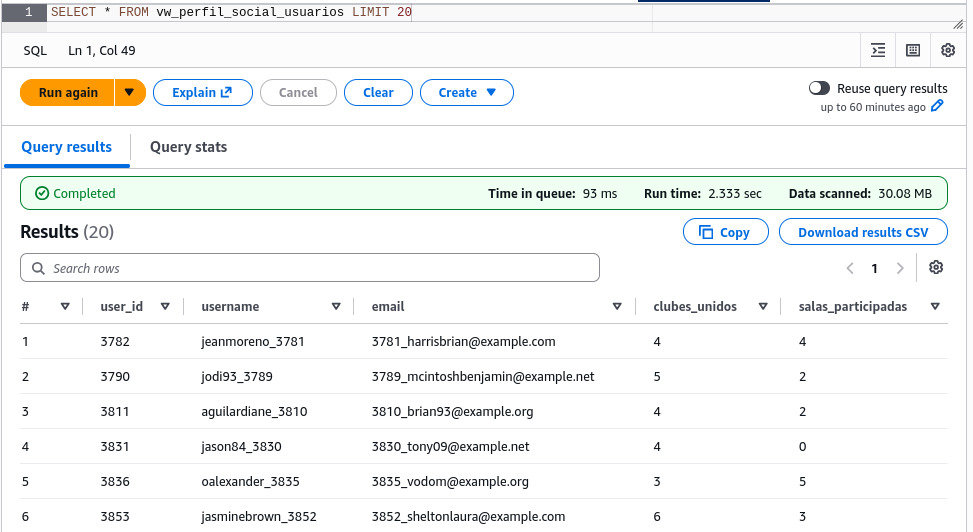
\includegraphics[width=.96\textwidth]{evidence/athena-vista2-consulta.jpeg}
  \caption{Consulta de la vista vw\_perfil\_social\_usuarios en AWS Athena}
\label{fig:athena-vista2-consulta}
\end{figure}

El flujo de datos parte de S3, donde \texttt{astra-crawler} registra la estructura en la base \texttt{astra\_analytics}; el modelo de la Figura~\ref{fig:modelo_datos_athena} representa las relaciones entre las tablas catalogadas y posteriormente consultadas mediante Athena.
\begin{figure}[H]\centering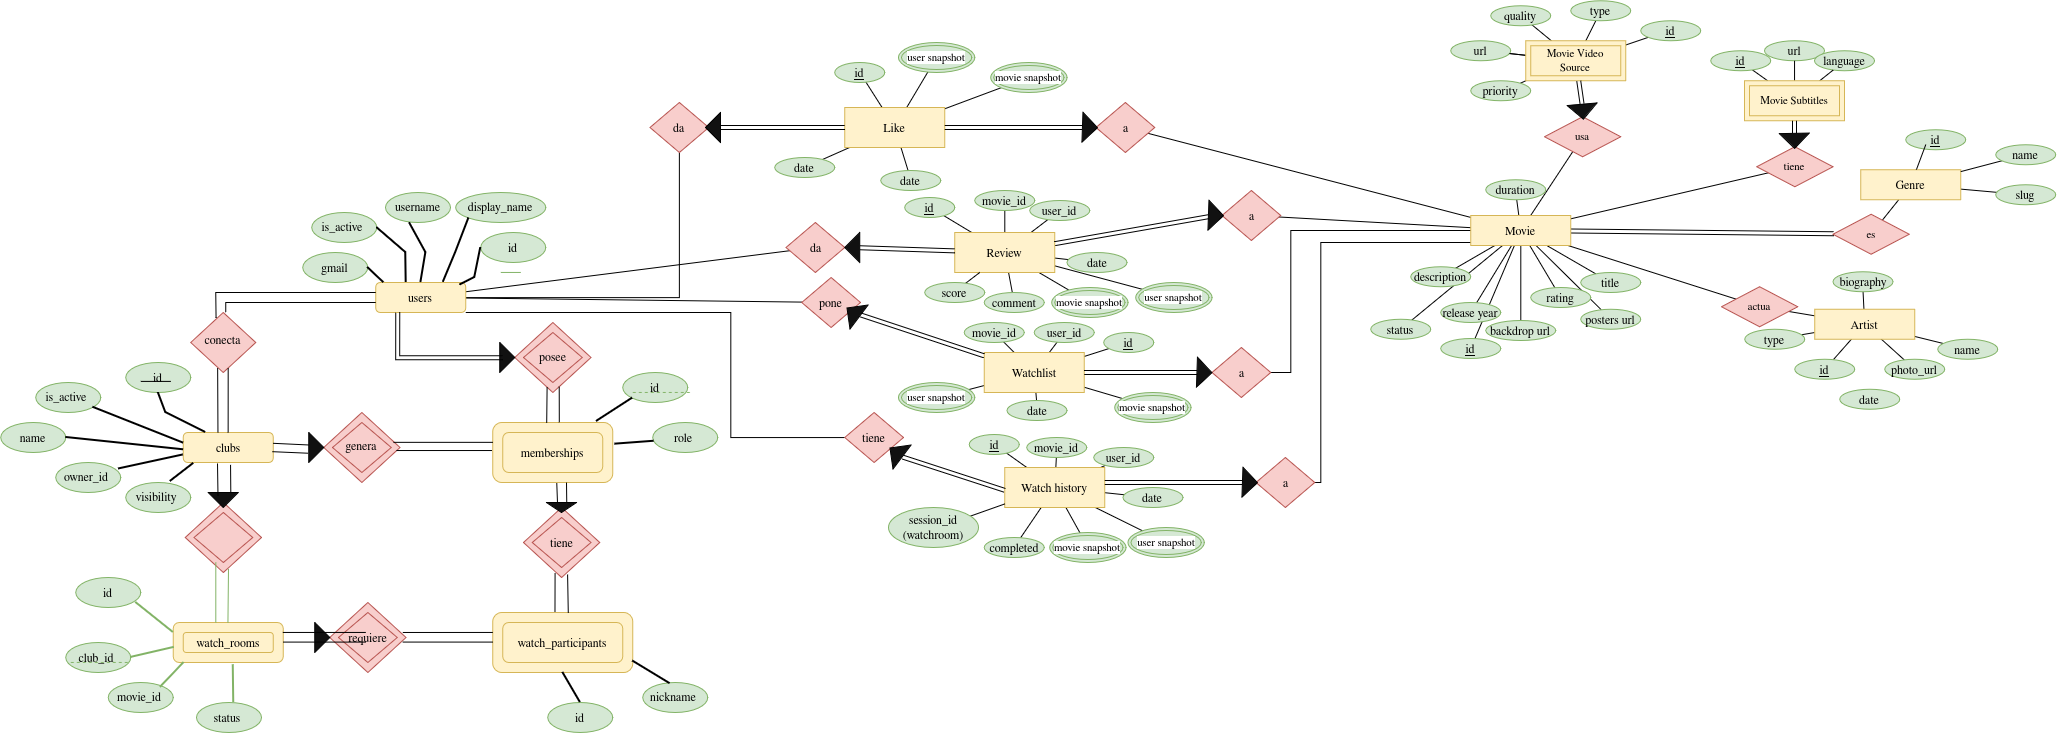
\includegraphics[width=\textwidth,height=.72\textheight,keepaspectratio]{../modelo_ER_Athena.png}\caption{Modelo de datos analítico consultado mediante Amazon Athena.}\label{fig:modelo_datos_athena}\end{figure}
